\chapter{Verificações, validações e análises}\label{Algumas_verificacoes_validacoes}

\section{Validação referente ao endurecimento e amolecimento da parte elastoplástica através de um ensaio}

Uma vez que se tem um ensaio triaxial, como por exemplo, o da \autoref{ensaio_triaxial_ductil} uma validação do endurecimento e amolecimento da parte elastoplástica é possível. Os modelos estão apresentados na \autoref{malha_ensaio_triaxial} e compreendem a simulação numérica de um ensaio considerando um modelo 3D, estado plano de deformação e axissimétrico. Sendo $l_a = l_b = l_c = 1$ o próprio deslocamento em y do nó A será a deformação específica. Para representar o ensaio da \autoref{ensaio_triaxial_ductil} foi aplicado um deslocamento imposto $\delta = 0.1$ em toda a face superior.

\begin{figure}[H]
	\begin{center}
		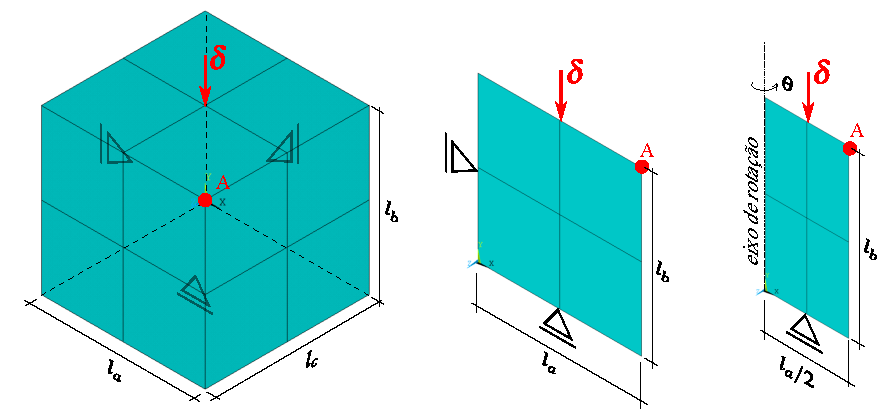
\includegraphics[scale = 1.0]{0701-Malha_ensaio_triaxial.pdf}
	\end{center}
	\caption{\label{malha_ensaio_triaxial}Domínio e discretização de um ensaio triaxial com modelo 3D, EPD e AXI}
\end{figure}

Os valores dos parâmetros do modelo constitutivo adotado na análise foram $E = 403$MPa, $\nu = 0,39$,  superficief = 2, superficieg = 2, $\phi = 0,~\psi = 0,~c_i = 0,7MPa,~c_p = 1,3MPa,~c_r = 0,9MPa,~\bar \varepsilon^p_{I} = 0,010,~\bar \varepsilon^p_{II} = 0,050,~\bar \varepsilon^p_{r} = 0,07$. Os parâmetros de coesão e de deformação plástica equivalente das zonas de endurecimento e amolecimento são coletados do gráfico do ensaio, tal como apresentado na \autoref{ensaio_triaxial_parametros}. O valor de duas vezes a coesão está no fato de que não está sendo considerado o ângulo de atrito, fazendo com que a superfície de plasticidade se reduza a de von-Mises. Também está sendo desconsiderado a dilatância, portanto, a variação do volume não considera a dilatância durante a deformação plástica. A parte viscosa do modelo constitutivo é eliminada utilizando uma coesão alta. O resultado da análise pode ser visto na \autoref{ensaio_triaxial_solucao}.
 
\begin{figure}[H]
 	\begin{center}
 		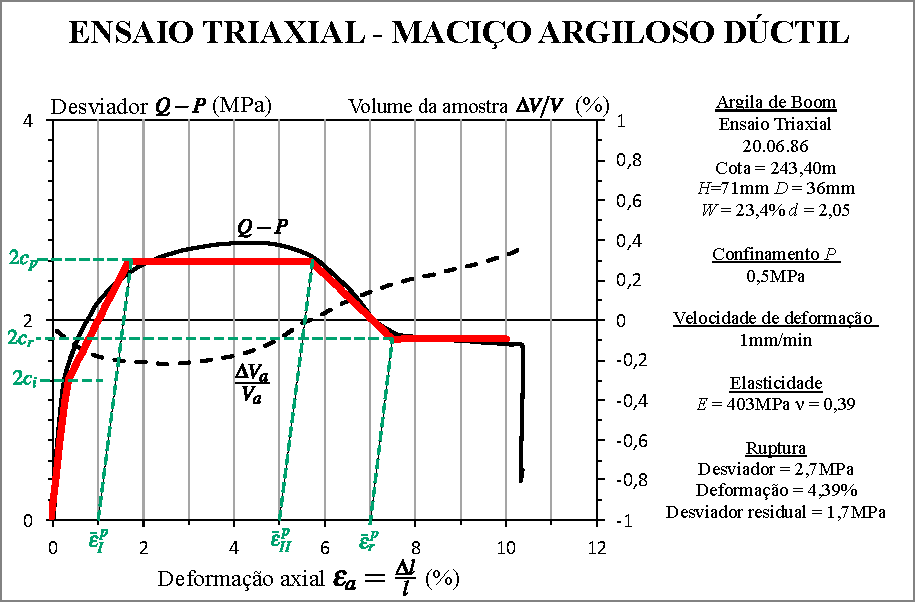
\includegraphics[scale = 0.9]{0702-ensaio triaxial argila ductil_coletando_parametros.pdf}
 	\end{center}
 	\caption{\label{ensaio_triaxial_parametros}Domínio e discretização de um ensaio triaxial com modelo 3D, EPD e AXI}
\end{figure}

\begin{figure}[H]
	\begin{center}
		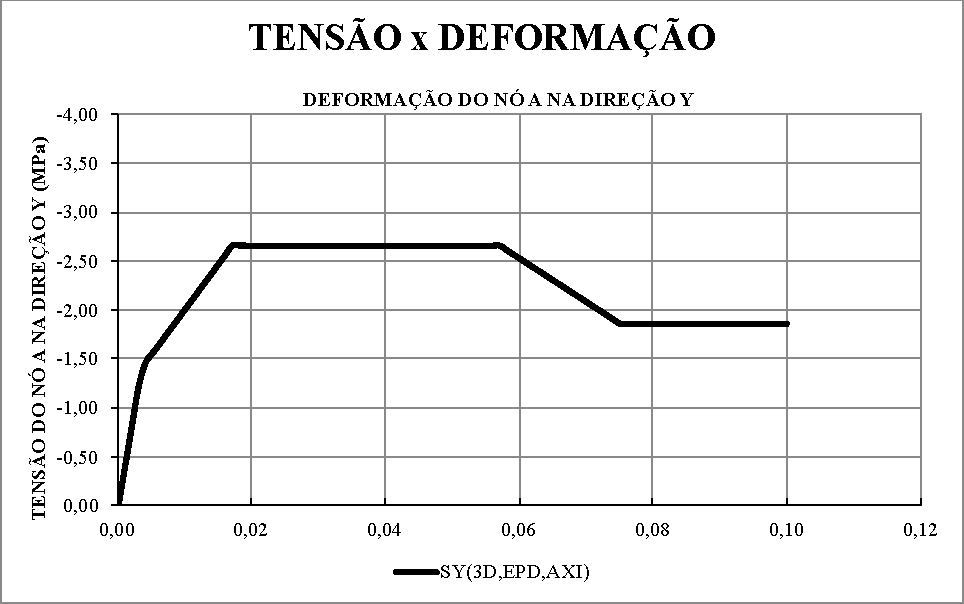
\includegraphics[scale = 1.0]{0703-ensaio triaxial argila ductil solucao.pdf}
	\end{center}
	\caption{\label{ensaio_triaxial_solucao}Resultado da análise para o ensaio triaxial}
\end{figure}

Como pode-se ver os valores deram exatamente iguais considerando 3D, EPD e AXI demonstrando que a implementação conseguiu essa generalidade. Caso o modelo seja de fato utilizado para estudos de túneis reais é sempre desejável ter ensaios triaxiais para fazer uma validação ou eventuais calibrações nesse aspecto do modelo.

\section{Verificação da solução numérica com uma solução analítica considerando o endurecimento}

Essa verificação considerará uma das soluções analíticas deduzidas por \citeonline{Bernaud2020}. A solução analítica escolhida corresponde a um problema de um túnel profundo de seção circular sobre tensão geostática hidrostática com um critério de plasticidade de Tresca considerando endurecimento por deformação plástica, conforme \autoref{coesao_solucao_analitca_LAJSS}. 

\begin{figure}[H]
	\begin{center}
		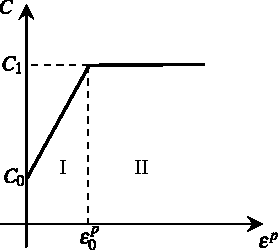
\includegraphics[scale = 1.2]{0704-lei de endurecimento ou amolecimento_coesao_solucao_analitca.pdf}
	\end{center}
	\caption{\label{coesao_solucao_analitca_LAJSS}Variação da coesão: I - trecho de endurecimento linear e II - comportamento perfeitamente plástico ( \citeonline[p.  4]{Bernaud2020})}
\end{figure}
A expressão (\ref{eq:LAJSS1}) apresenta a solução analítica da convergência quando $r=R_i$.
\begin{equation}
	\label{eq:LAJSS1}
	\dfrac{u(r)}{r} = \dfrac{(1-2\nu)(\nu+1)}{E}\left\{\sigma_x+\dfrac{2C_0}{1+2\dfrac{C'}{E'}}\left[\dfrac{C'}{E'}\left(\dfrac{1}{r^2}-\dfrac{1}{x^2}\right) y^2+\ln{\left(\dfrac{x}{r}\right)-\sigma_\infty} \right]  \right\}-\dfrac{2C_0}{E'}\left(\dfrac{y}{r}\right)^2
\end{equation}
em que $E'=E/(1+\nu),~\nu,~C' = (C_1-C_0)/\varepsilon_0^p$ são parâmetros do material. Essa solução é dependente também dos raios plásticos $x,~y$, da tensão na fronteira do raio plástico $\sigma_x$, das tensões geostáticas hidrostáticas $\sigma_\infty$ e da tensão no interior da cavidade do túnel $\sigma_i$. O restante das expressões para aplicar essa solução são:
\begin{equation} \label{eq:LAJSS2}
	{{\sigma }_{x}}=2{{C}_{1}}\ln \left( \frac{{{R}_{i}}}{x} \right)+{{\sigma }_{i}},~~~ 	{{x}^{2}}=\frac{2{{C}_{0}}}{E'\varepsilon _{0}^{p}+2{{C}_{1}}}{{y}^{2}}, ~~~ 	{{y}^{2}}=\frac{{{R}_{i}}}{{{\omega }_{0}}}{{e}^{\frac{({{\omega }_{1}}+{{\omega }_{2}}+{{\omega }_{3}})}{{{C}_{1}}}}} 
\end{equation}
\begin{equation} \label{eq:LAJSS3}
	{{\omega }_{0}}=\frac{2{{C}_{0}}}{E'\varepsilon _{0}^{p}+2{{C}_{1}}}, ~~~ 	{{\omega }_{1}}={{\sigma }_{i}}-{{\sigma }_{\infty }}-{{C}_{0}} , ~~~ {{\omega }_{2}}=\frac{{{C}_{0}}}{1+2\frac{C'}{E'}}\ln ({{\omega }_{0}}), ~~~ 	{{\omega }_{3}}=\frac{\frac{C'}{E'}\left[ 2({{C}_{0}}-{{C}_{1}})-\varepsilon _{0}^{p} \right]}{1+2\frac{C'}{E'}}
\end{equation}

Utilizando $R_i=1$m, $E=1430$MPa, $\nu = 0,4$, $C_0=0,21$MPa, $C_1=0,56$MPa, $\varepsilon _{0}^{p}=0,024$, $P_i = -\sigma_i = 2,5$MPa, $ P_\infty = -\sigma_\infty = 4,5$MPa tem-se, pela expressão analítica, $U_i(\%) = - u(r=R_i)/R_i = 5,91$. A \autoref{solucao_numérica_LAJSS} apresenta a concordância do resultado numérico com um erro menor que 1\%.

\begin{figure}[H]
	\begin{center}
		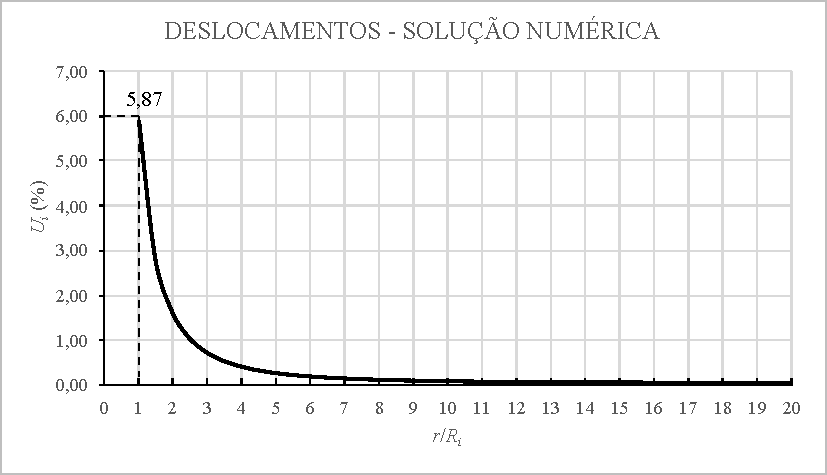
\includegraphics[scale = 1.0]{0705-lei de endurecimento ou amolecimento_coesao_solucao_numerica.pdf}
	\end{center}
	\caption{\label{solucao_numérica_LAJSS}Solução numérica considerando elastoplasticidade com endurecimento}
\end{figure}
Para essa solução numérica foi utilizado domínio em EPD (\autoref{malhaEPD_tunel}) e a relação (\ref{eq:ctr_cvm})$_1$ que considera a superfície de von-Mises inscrita em Tresca e as mesmas considerações para particularizar o modelo elastoplástico-viscoplástico para elastoplástico, ou seja, a parte viscosa do modelo constitutivo é novamente eliminada utilizando uma coesão viscosa alta. Para representar a mesma lei de endurecimento tem-se $c_i = 0,21\sqrt{3}/2$, $c_p = 0,56\sqrt{3}/2$, $c_r = 0,56\sqrt{3}/2,~\bar \varepsilon^p_{I} = 0,024,~\bar \varepsilon^p_{II} = 0,024,~\bar \varepsilon^p_{r} = 0,024$. 

\section{Verificação do modelo acoplado com cada comportamento em separado}
O modelo constitutivo elastoplástico-viscoplástico é bastante geral e capaz de reproduzir cada comportamento em separado. Portanto, é apresentado algumas verificações da solução numérica considerando cada lei constitutiva separada: I - elasticidade, II - elastoplasticidade e III - viscoplasticidade. Para o caso I e II sem revestimento é utilizado soluções analíticas como comparação. A expressão dessas podem ser encontradas em \citeonline{Corbeta1990} e \citeonline[p. 50-54]{Quevedo2017} e portanto não serão apresentadas. A solução elastoplástica considera uma plasticidade perfeita com regra de fluxo associada com superfície de escoamento de Tresca. Portanto é utilizado a relação (\ref{eq:ctr_cvm})$_1$. Para outros casos e quando se tem revestimento a verificação foi feita com outro \textit{software}, o GEOMEC91. O GEOMEC91 é um programa de elementos finitos para geomecânica para análises bidimensionais em axissimetria. Ele foi desenvolvido por \citeonline{Bernaud1991} e detalhes de sua malha e condições de contorno podem ser vistas em \citeonline[p. 190]{Bernaud1991}.

Os resultados apresentados nessa seção são os do modelo axissimétrico da \autoref{malhaAXI_tunel} com os parâmetros da \autoref{parametros_AXI}. Apesar de estar limitado às condições de axissimetria, é um dos modelos mais importantes, pois considera o processo de escavação e colocação do revestimento de forma realista e permite fazer estudos paramétricos de forma mais eficiente que os modelos tridimensionais. Contudo, as mesmas verificações foram feitas no modelo tridimensional considerando seção circular e os mesmos resultados foram obtidos, com pequenas diferenças menores que 1\%.

\subsection{Verificações em elasticidade}

O modelo constitutivo acoplado, por ser geral, tem que ser capaz de reproduzir o resultado em elasticidade colocando coesões elevadas na parte plástica e viscosa. Dessa forma, considerando $E =$1000MPa e 5000MPa, $\nu =$ 0.498MPa, $p_v = p_h = 5$MPa tem-se os resultados da \autoref{ELAST-D0-E1000-ER0-P5} e \autoref{ELAST-D0-E5000-ER0-P5}. As curvas cinzas são os perfis de convergência a cada passo de escavação e a vermelha no último passo. A curva verde pontilhada é a solução analítica.

\begin{figure}[H]
	\begin{center}
		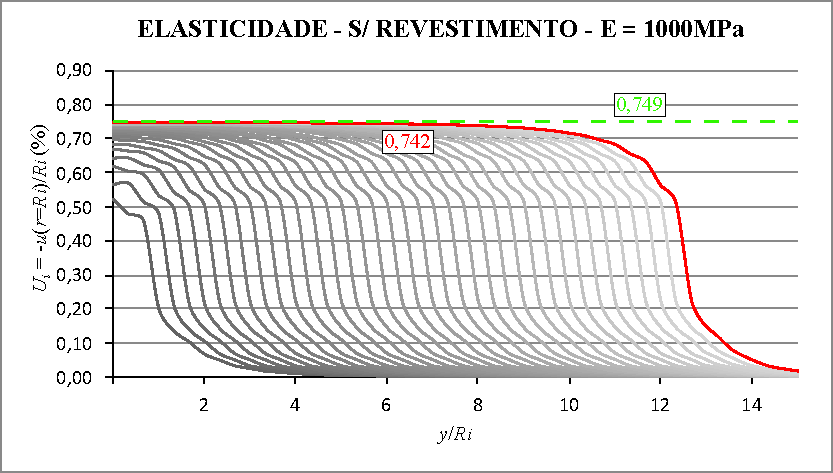
\includegraphics[scale = 1.0]{0706-AXI-SREVESTIMENTO-E1000.pdf}
	\end{center}
	\caption{\label{ELAST-D0-E1000-ER0-P5}Verificação solução numérica em elasticidade sem revestimento - E = 1000MPa}
\end{figure}

\begin{figure}[H]
	\begin{center}
		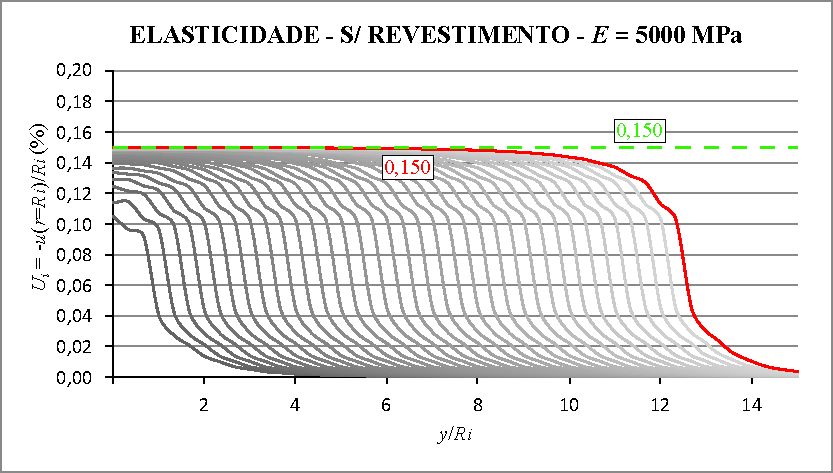
\includegraphics[scale = 1.0]{0707-AXI-SREVESTIMENTO-E5000.pdf}
	\end{center}
	\caption{\label{ELAST-D0-E5000-ER0-P5}Verificação solução numérica em elasticidade sem revestimento - E = 5000MPa}
\end{figure}

Cabe salientar que quando se utiliza o modelo constitutivo elástico linear a mesma solução é obtida escavando todos os passos de uma única vez. Contudo, quando se tem revestimento não há solução analítica, pois ocorre a iteração entre o revestimento e o maciço. Para essa verificação é comparado o resultado do ANSYS com o GEOMEC91. A \autoref{ELAST-D0-E1000-ER30000-P5} mostra essa comparação considerando $E$ = 1000MPa com um revestimento de $E_{rev}$=30000MPa e $\nu_{rev}$ = 0,3. Nesse caso, foi considerado um $d0$ = 0.

\begin{figure}[H]
	\begin{center}
		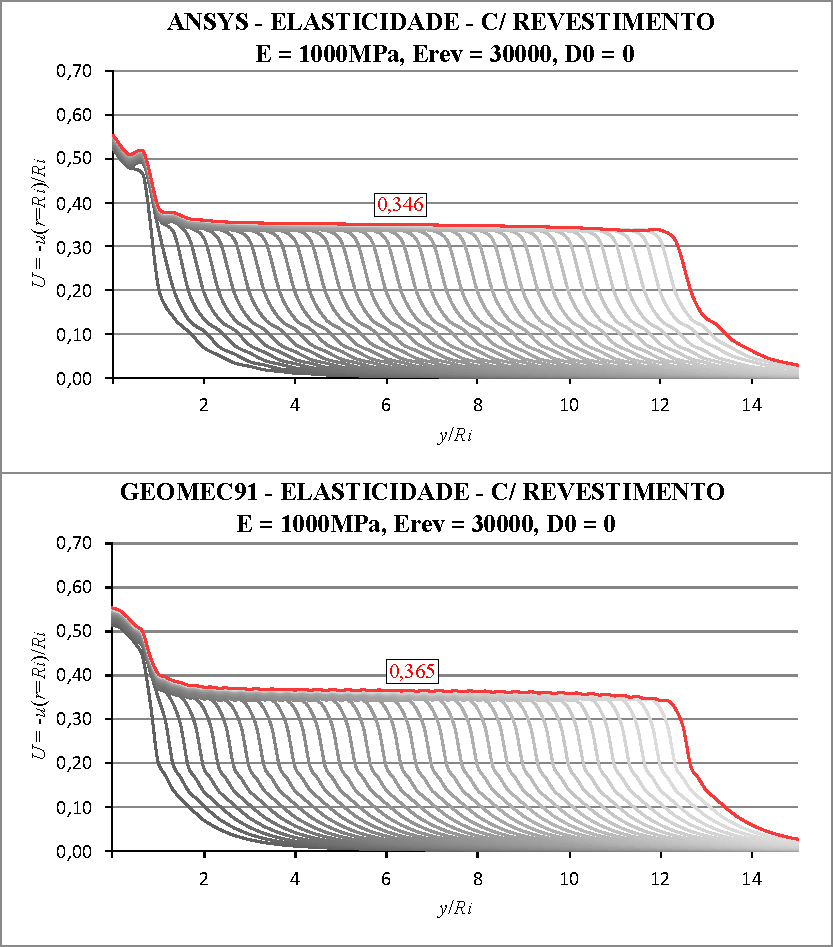
\includegraphics[scale = 1.0]{0708-AXI-SREVESTIMENTO-E1000-ER30000-D0.pdf}
	\end{center}
	\caption{\label{ELAST-D0-E1000-ER30000-P5}Verificação solução numérica em elasticidade com revestimento - $E$ = 1000MPa, $E_{rev}$ = 30000MPa, $d0$ = 0}
\end{figure}

O perfil de convergência apresenta um pico nas primeiras escavações, uma vez que na primeira escavação é escavado 3$L_p$. De qualquer forma, em comparação com a \autoref{ELAST-D0-E1000-ER0-P5} consegue-se ver que o revestimento tem um grande efeito sobre as deformações. Nesse caso, a rigidez do revestimento é muito elevada em relação ao maciço. Contudo, não é só o módulo de elasticidade do revestimento que conta, mas tão importante quanto, o d0. Considerando um $d_0=4L_p$ tem-se os resultados da \autoref{ELAST-D4-E1000-ER30000-P5}.

\begin{figure}[H]
	\begin{center}
		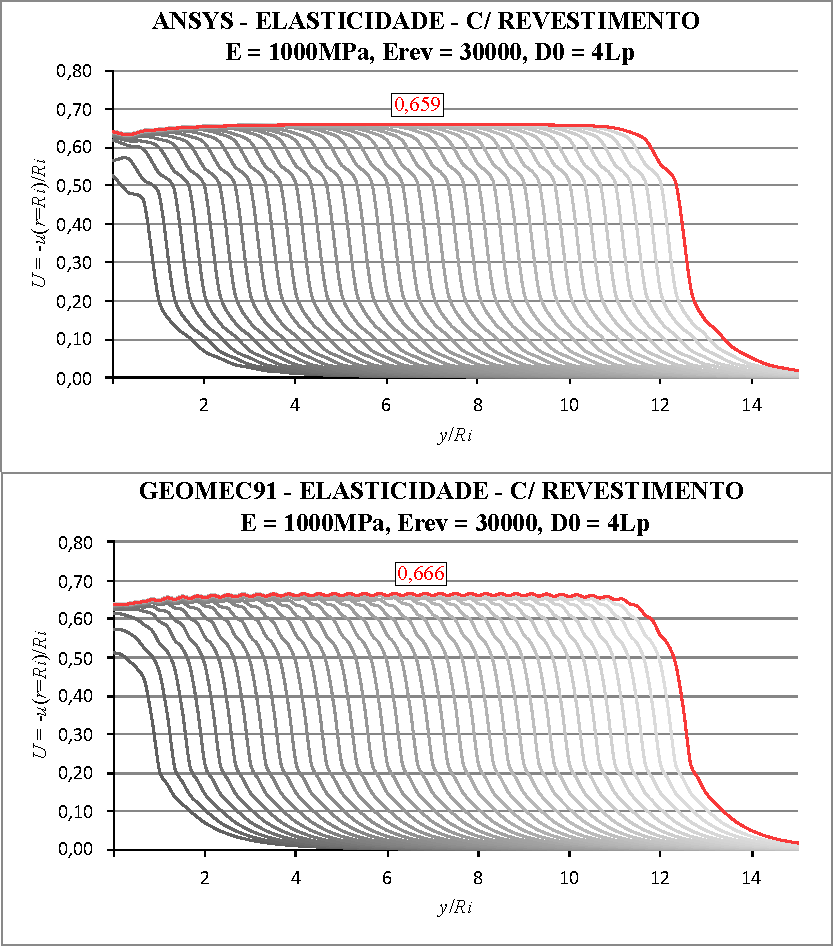
\includegraphics[scale = 1.0]{0709-AXI-SREVESTIMENTO-E1000-ER30000-D4.pdf}
	\end{center}
	\caption{\label{ELAST-D4-E1000-ER30000-P5}Verificação solução numérica em elasticidade com revestimento - $E$ = 1000MPa, $E_{rev}$ = 30000MPa, $d0$ = 4$L_p$}
\end{figure}

Na \autoref{ELAST-D4-E1000-ER30000-P5} pode-se ver pequenas ondulações no perfil de convergências do GEOMEC91 que não estão presentes no resultado do ANSYS. Essa diferença ocorre devido ao elemento finito utilizado. No GEOMEC91 é utilizado um elemento quadrático, que possuí um nó intermediário em suas bordas.

Como pode-se notar o modelo constitutivo acoplado conseguiu em elasticidade reproduzir outras soluções independentes. Ademais, a verificação do modelo em elasticidade é muito importante para conferir se as escavações e a colocação do revestimento estavam sendo feitas corretamente. Além disso, deram uma ideia inicial da qualidade da malha.

\subsection{Verificações em elastoplasticidade}

De forma análoga à elasticidade, o modelo constitutivo acoplado, por ser um modelo de aplicação geral, tem que ser capaz de reproduzir o resultado em elastoplasticidade utilizando uma coesão viscoplástica elevada. Considerando $E =$1000MPa, $\nu =$ 0,498MPa, $p_v = p_h = 4$MPa, $c_i=c_p=c_r = \sqrt{3}/2$MPa e $3\sqrt{3}/2$MPa  tem-se os resultados da \autoref{PLAST-D0-E1000-ER0-P4-C1} e \autoref{PLAST-D0-E1000-ER0-P4-C3}. As curvas cinzas são os perfis de convergência a cada passo de escavação e a vermelha no último passo. A curva verde pontilhada é a solução analítica.

\begin{figure}[H]
	\begin{center}
		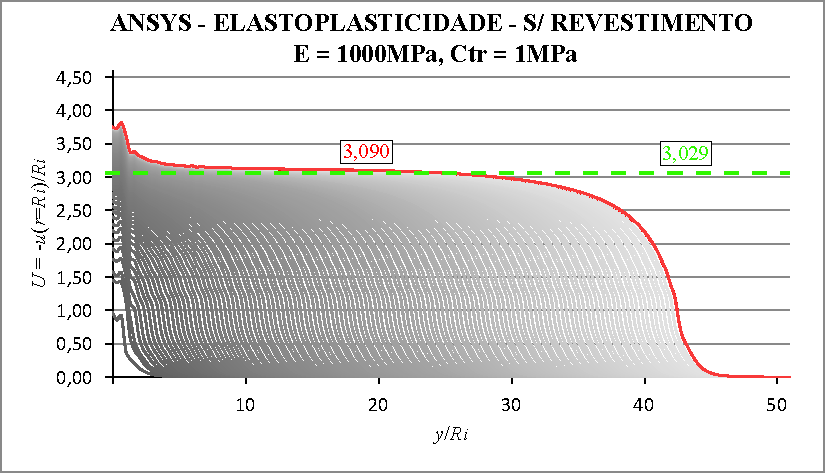
\includegraphics[scale = 1.0]{0710-AXI-PLAST-SREVESTIMENTO-D0-E1000-ER0-P4-C1.pdf}
	\end{center}
	\caption{\label{PLAST-D0-E1000-ER0-P4-C1}Verificação solução numérica em elastoplasticidade sem revestimento - $E$ = 1000MPa,  $c_i=c_p=c_r = \sqrt{3}/2$MPa}
\end{figure}
No caso em que $c_i=c_p=c_r = \sqrt{3}/2$MPa, foi necessário aumentar o número de passos de escavação $n_p = 128$ para que o patamar no perfil de convergência se desenvolvesse plenamente. A solução analítica é dada para esse patamar sem a influência da face de escavação ou das bordas do modelo. Isso demonstra que dependendo dos valores dos parâmetros constitutivos pode ser necessário aumentar o número de passos $n_p$. Se o valor almejado é a convergência no equilíbrio fora das zonas de influência deve-se buscar uma malha suficiente para aparecer o patamar no perfil de convergências. Um outro aspecto em que o domínio deve ser ajustado é quando as deformações plásticas alcançam suas fronteiras, sendo nesse caso necessário aumentar o limites do domínio ($L_x,~L_y$ e $L_z$). Para o domínio escolhido resultados são obtidos de forma satisfatória sempre que a relação da pressão geostática-hidrostática pela coesão for menor ou igual a 5. Caso contrário, pode ser necessário fazer esse ajuste nas fronteiras do domínio.
\begin{figure}[H]
	\begin{center}
		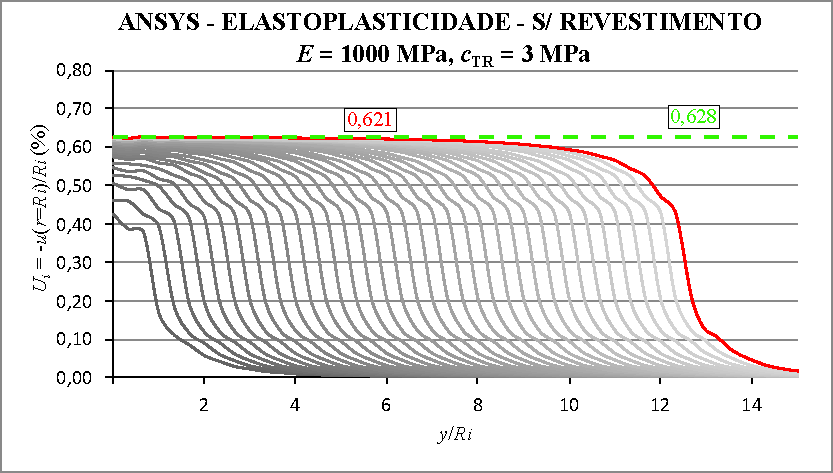
\includegraphics[scale = 1]{0711-AXI-PLAST-SREVESTIMENTO-D0-E1000-ER0-P4-C3.pdf}
	\end{center}
	\caption{\label{PLAST-D0-E1000-ER0-P4-C3}Verificação solução numérica em elastoplasticidade sem revestimento - $E$ = 1000MPa, $c_i=c_p=c_r = 3\sqrt{3}/2$MPa}
\end{figure}
 A próxima verificação, compreende a plasticidade dependente da pressão e não associada. Para tanto é utilizado um ângulo de atrito $\phi$=15$^\circ$ e um ângulo de dilatância $\psi$=0$^\circ$. O resultado pode ser visto na \autoref{PLAST-D0-E1000-ER0-P4-C1-KP15-KB1}. Essa solução apenas não converge quando se utiliza Newton-Raphson Completo com o módulo constitutivo consistente. Se for utilizar o módulo constitutivo consistente é necessário utilizar o Newton-Raphson Completo Assimétrico. A opção em que é utilizado Newton-Raphson Completo mas sem atualizar o módulo constitutivo converge para a solução. Outro aspecto importante, comparando o resultado da \autoref{PLAST-D0-E1000-ER0-P4-C1-KP15-KB1} com a \autoref{PLAST-D0-E1000-ER0-P4-C1} é a sensibilidade com que a convergência é afetada pelo ângulo de atrito. Esse resultado é esperado uma vez que quanto maior o ângulo de atrito, para uma dada pressão hidrostática, mais afastada fica a superfície de plastificação do eixo hidrostático.
\begin{figure}[H]
	\begin{center}
		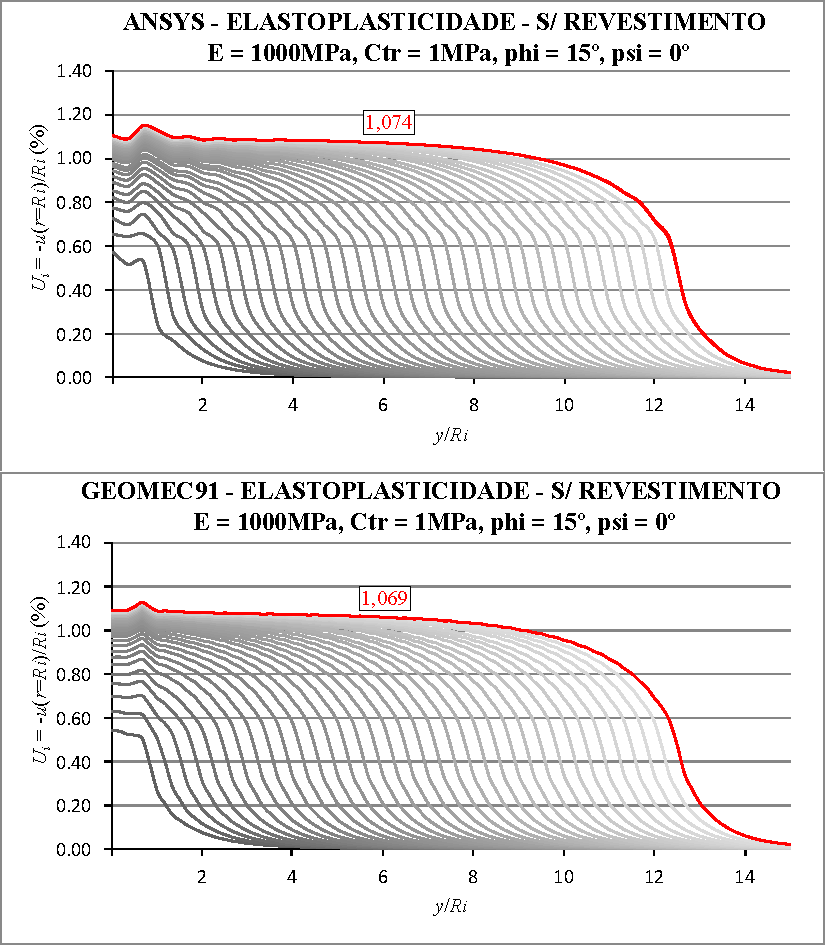
\includegraphics[scale = 1]{0712-AXI-PLAST--D0-E1000-ER0-P4-C1-KP15-KB1.pdf}
	\end{center}
	\caption{\label{PLAST-D0-E1000-ER0-P4-C1-KP15-KB1}Verificação solução numérica elastoplasticidade sem revestimento $E$ = 1000MPa, $c_i=c_p=c_r = \sqrt{3}/2$MPa, $\phi$=15$^\circ$ e $\psi$=0$^\circ$}
\end{figure}

A verificação da solução considerando a colocação de um revestimento com $E_{rev} = 30000$MPa, $\nu_{rev} = 0,3$ e $d_0=0$ pode ser vista na \ref{PLAST-D0-E1000-ER30000-P4-C1}.

\begin{figure}[H]
	\begin{center}
		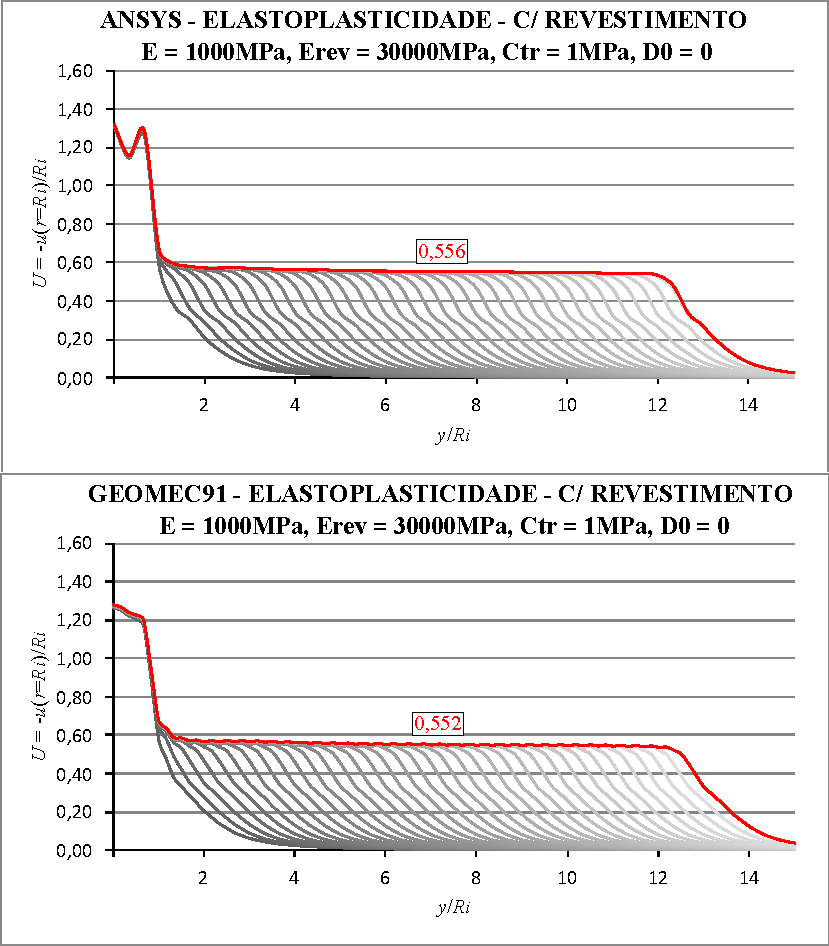
\includegraphics[scale = 1.0]{0713-PLAST-D0-E1000-ER30000-P4-C1.pdf}
	\end{center}
	\caption{\label{PLAST-D0-E1000-ER30000-P4-C1}Verificação solução numérica em elastoplasticidade com revestimento - $E$ = 1000MPa, $E_{rev}$ = 30000MPa, $d0=0$, $c_i=c_p=c_r=\sqrt{3}/2$}
\end{figure}

\subsection{Verificações em viscoplasticidade}

De forma análoga à elasticidade e à elastoplasticidade, o modelo constitutivo acoplado, por ser geral, tem que ser capaz de reproduzir o resultado viscoplástico colocando coesões elevadas na parte elastoplástica.  Considerando $E =$1000MPa, $\nu =$ 0,498MPa, $p_v = p_h = 4$MPa, $c_i=c_p=c_r = \sqrt{3}/2$MPa, $V_p = 5$m/dia tem-se os resultados da \autoref{VISCO-D0-E1000-ER0-P4-C1-V5}. As curvas cinzas abaixo da curva vermelha são os perfis de convergência a cada passo de escavação. A curva vermelha o perfil de convergência da última escavação e colocação do revestimento. A curva azul é o perfil de convergência após os efeitos viscosos cessarem. As curvas cinzas entre a curva vermelha e azul mostram a evolução do perfil de convergências a cada intervalo de tempo, que está indicado no gráfico.
\begin{figure}[H]
	\begin{center}
		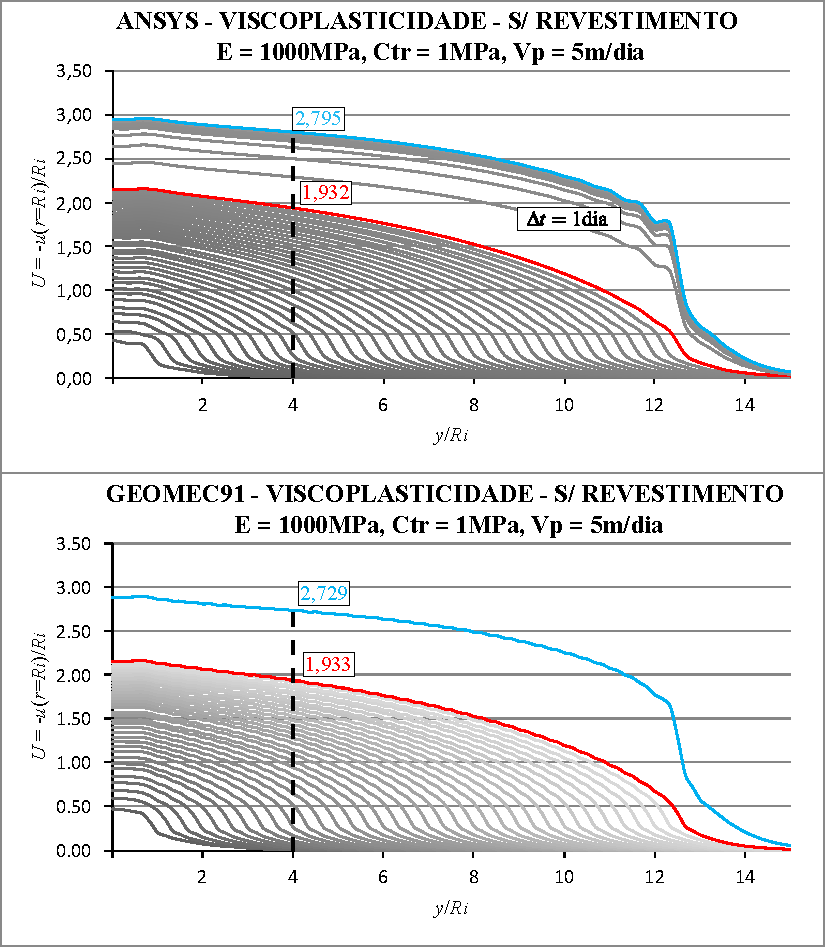
\includegraphics[scale = 1.0]{0714-AXI-D0-E1000-ER0-P4-C1-V5.pdf}
	\end{center}
	\caption{\label{VISCO-D0-E1000-ER0-P4-C1-V5}Verificação solução numérica em elastoplasticidade com revestimento - $E$ = 1000MPa, $c_i=c_p=c_r=\sqrt{3}/2$, $V_p=5$m/dia}
\end{figure}
Como pode-se ver o resultado do GEOMEC91 não apresenta a evolução do perfil de convergências entre o final da construção do túnel e o final dos efeitos viscosos (longo prazo). Contudo, o longo prazo é quando o perfil de convergências cessa sua evolução. Isso pode ser visto no modelo do ANSYS pela aproximação das curvas cinzas entre a curva vermelha e azul conforme o tempo passa. Outro aspecto é que, para esses parâmetros, a quantidade de escavação $n_p$ não foi suficiente para aparecer o patamar no perfil de convergências, portanto os valores escolhidos para comparação estão na cota $y/R_i=4$. Um aspecto importante a ser notado é que quando se tem apenas viscoplasticidade, sem revestimento, o perfil de convergências no longo prazo tende a se aproximar da solução elastoplástica com os parâmetros do modelo viscoso, como pode ser visto comparando a \autoref{VISCO-D0-E1000-ER0-P4-C1-V5} e \autoref{PLAST-D0-E1000-ER0-P4-C1}. Além disso, o perfil de convergências no final da construção do túnel (curto prazo), tende a se aproximar da solução em elasticidade (menores convergências) quando a velocidade de escavação $V_p$ aumenta. A \autoref{VISCO-D0-E1000-ER0-P4-C1-V10} mostra esse aspecto com uma velocidade de 10m/dia.

\begin{figure}[H]
	\begin{center}
		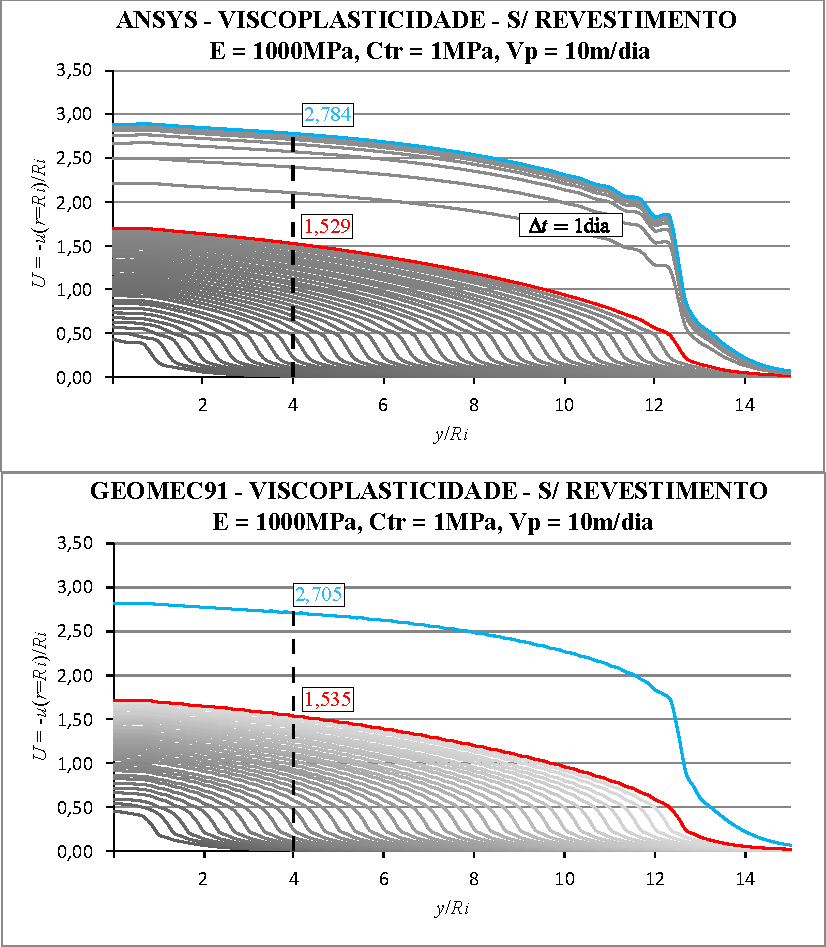
\includegraphics[scale = 1.0]{0715-AXI-D0-E1000-ER0-P4-C1-V10.pdf}
	\end{center}
	\caption{\label{VISCO-D0-E1000-ER0-P4-C1-V10}Verificação solução numérica em viscoplasticidade com revestimento - $E$ = 1000MPa, $c_i=c_p=c_r=\sqrt{3}/2$, $V_p=10$m/dia}
\end{figure}
Como pode-se ver o perfil de convergências no longo prazo não sofreu alteração e o perfil de curto prazo diminuiu suas convergências. \textbf{O modelo constitutivo acoplado traz diferença justamente nesse aspecto}: a convergência no curto prazo será influenciada por eventuais plastificações e a convergência de longo prazo não terá mais esse comportamento de se aproximar da solução elastoplástica com os mesmos valores dos parâmetros viscosos.

Por fim, para verificar a parte do modelo viscoplástico com revestimento a \autoref{VISCO-D2-E1000-ER3000-P4-C1-V5} apresenta uma comparação considerando um revestimento de $E_{rev}=3000$MPa, $\nu_{rev}=0,3$ colocado com $d_0=2L_p$ afastado da face de escavação.

\begin{figure}[H]
	\begin{center}
		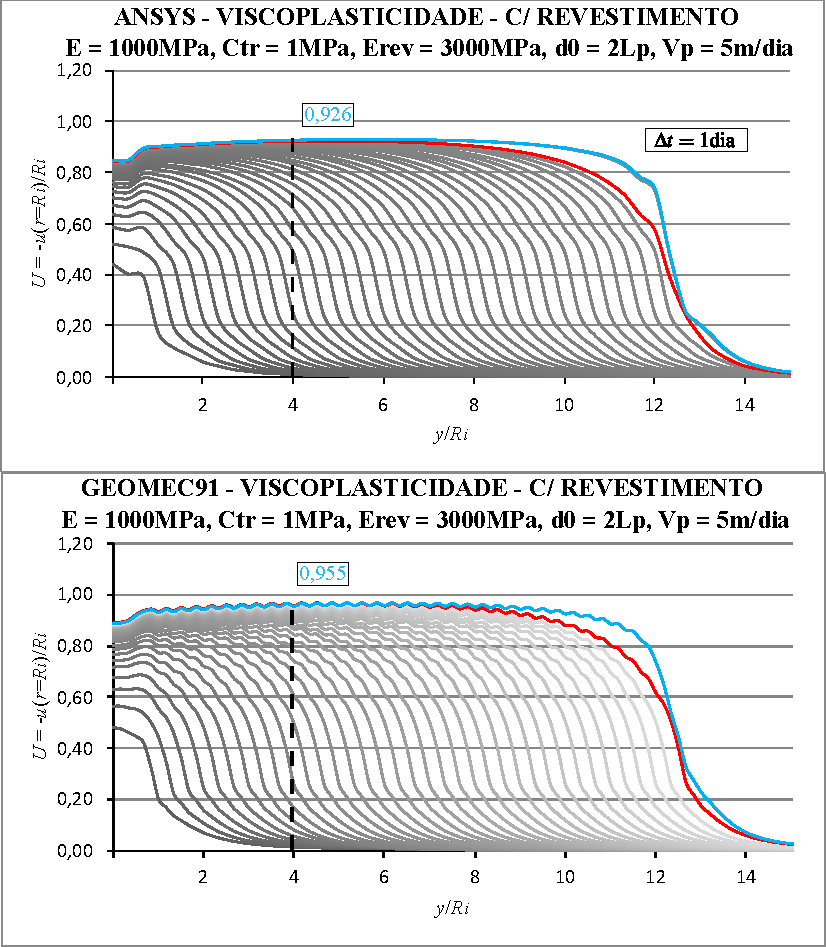
\includegraphics[scale = 1.0]{0716-AXI-D2-E1000-ER3000-P4-C1-V5.pdf}
	\end{center}
	\caption{\label{VISCO-D2-E1000-ER3000-P4-C1-V5}Verificação solução numérica em viscoplasticidade com revestimento - $E$ = 1000MPa, $c_i=c_p=c_r=\sqrt{3}/2$, $E_{rev} = 3000$MPa, $d0=2L_p$, $V_p=5$m/dia}
\end{figure}
O revestimento, de uma forma geral, diminui as convergências tanto de curto quanto de longo prazo resistindo as deformações. Contudo, quando se tem um revestimento viscoso, como o concreto que sofre fluência e retração, esse bloqueio não é tão eficiente como pode ser visto em \citeonline{Quevedo2017}. Além disso, a baixa rigidez do revestimento faz com que o perfil de convergências no final da construção do túnel (curto prazo) se aproxime do de longo prazo.

\section{Verificação do modelo elastoplástico-viscoplástico com uma solução analítica}

De modo a verificar o algoritmo acoplado implementado é feita a comparação com a solução analítica deduzida por \citeonline[p. 61]{Piepi1995} para um túnel profundo em condições geostáticas-hidrostáticas no interior de um maciço com comportamento elastoplástico-viscoplástico perfeito obedecendo ao critério de Tresca. Essa solução analítica foi escolhida por utilizar o mesmo princípio de associação da \autoref{lei_endurecimento_rousset}, como pode ser visto em \citeonline[p. 35]{Piepi1995}. Contudo, não apresenta a mesma generalidade da solução numérica implementada e possui algumas hipóteses simplificativas, dentre elas, a consideração da mesma superfície de escoamento para plasticidade e viscoplasticidade e vetores de fluxo totalmente associados, ou seja, $\fl^p = \gl^{p} = \fl^{vp} = \gl^{vp}$. Para essa verificação é utilizado o modelo axissimétrico com os seguintes parâmetros: $E=1500$MPa e $2000$MPa, $\nu=0,498$, $c^i=c^p=c^r =4\sqrt{3}/2$MPa, $c^{vp}=3\sqrt{3}/2$MPa, $\eta = 4 \cdot 10^4$dia, $n=1$, $f_0=1$MPa e $p_v=p_h=9$MPa. Esses parâmetros são os mesmos utilizado por \citeonline[p. 131]{Piepi1995} que chegou nas convergências de $U=2,16$\% para $E=1500$MPa e $U=1,6$\% para $E=2000$MPa.

Como a solução analítica está deduzida para superfície de Tresca e aqui é utilizada a de Drucker-Prager (que se particulariza para von-Mises devido a ausência de ângulo de atrito) foi adotado a relação (\ref{eq:ctr_cvm})$_1$ considerando von-Mises inscrito em Tresca nos valores das coesões. A solução analítica obtém o perfil de convergência apenas no longo prazo. Contudo, para mostrar as diferenças entre os modelos, além da solução numérica elastoplástica-viscoplástica (EPVP), foi feita também a solução considerando cada comportamento separado, ou seja, elástico (E), elastoplástico (EP) e viscoplástico (VP) tanto no final da escavação quanto no longo prazo. O modelo viscoplástico (VP) é utilizada a mesma coesão de $4\sqrt{3}/2$ do modelo (EP). Para averiguar a influência da velocidade de escavação será considerado três velocidades $V_p=0,1; 0,2$ e 10m/dia.

A \autoref{PIEPI-E1500-FINALESCAVACAO} apresenta os resultados no final da escavação. Pode-se notar que os perfis de convergência para o modelo viscoplástico (VP) são intermediários entre o modelo elástico (E) e elastoplástico (EP), sendo que quanto mais rápida a escavação, mais a resposta desse modelo se  aproxima da convergência do maciço em elasticidade. Isso é um resultado esperado, pois quanto maior a velocidade de escavação menos tempo transcorreu para a evolução das deformações viscosas. O modelo elastoplástico-viscoplástico (EPVP) apresentou a mesma relação com a velocidade (quanto mais rápido menos tempo para as deformações viscosas evoluírem), porém, \textbf{iniciou suas deformações próximas do perfil de convergências do modelo elastoplástico (EP)}. Isso ocorre, pois, o maciço atingiu a plastificação durante a escavação. \textbf{Esse é um dos principais objetivos e vantagem desse modelo acoplado}, pois geralmente a escavação induz um comportamento elastoplástico no maciço próximo à abertura e esse efeito não é captado pelos modelos que consideram apenas a viscoplasticidade.

\begin{figure}[H]
	\begin{center}
		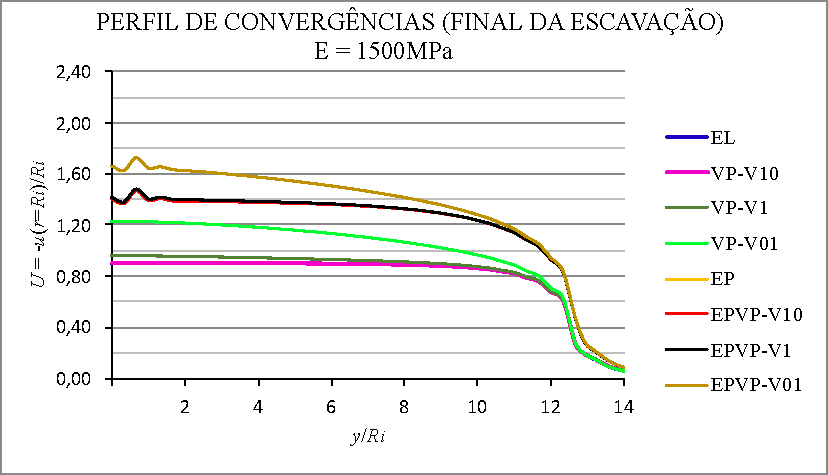
\includegraphics[scale = 1.0]{0717-PIEPI-E1500-FINALESCAVACAO.pdf}
	\end{center}
	\caption{\label{PIEPI-E1500-FINALESCAVACAO}Perfis de convergências no final da escavação para os diversos comportamentos implementados, considerando os parâmetros físicos do maciço de acordo com \citeonline{Piepi1995} com $E=1500$MPa}
\end{figure}

Após o final da escavação, os perfis de convergências dos modelos (VP) e (EPVP) continuam evoluindo com uma taxa cada vez menor devido a redistribuição de tensões no interior do maciço, até estabilizarem (no longo prazo). A \autoref{PIEPI-E1500-LONGOPRAZO} mostra os perfis de convergências no longo prazo (cerca de 500 dias). Pode-se ver que independente da velocidade de escavação, os perfis de convergêncais viscoplásticos (VP) se estabilizam sobre o perfil da elastoplasticidade (EP). Isso ocorre pois é utilizado a mesma superfície de escoamento com os mesmos parâmetros em ambos os modelos. Contudo, os perfis do modelo elastoplástico-viscoplástico (EPVP) encontram a estabilização bem acima do perfil do modelo elastoplástico (EP), o que mostra, mais uma vez a importância da magnitude desse comportamento acoplado. Pode-se ver também que a solução numérica no longo prazo ficou satisfatória com a solução analítica.

\begin{figure}[H]
	\begin{center}
		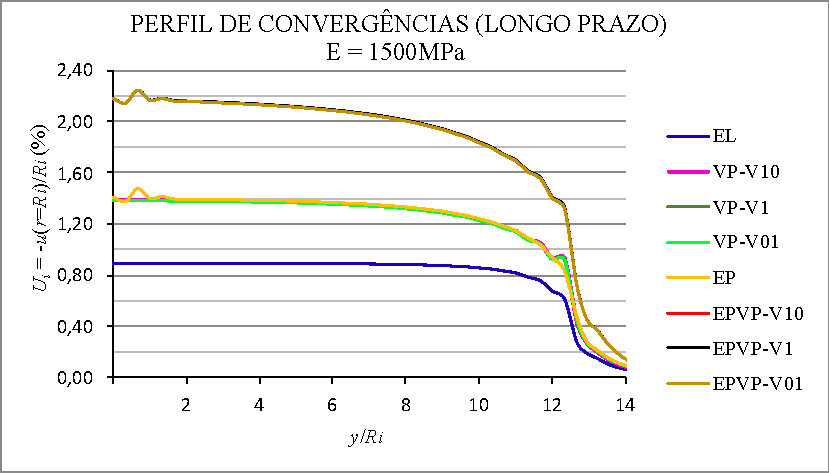
\includegraphics[scale = 1.0]{0718-PIEPI-E1500-LONGOPRAZO.pdf}
	\end{center}
	\caption{\label{PIEPI-E1500-LONGOPRAZO}Perfis de convergências no longo prazo para os diversos comportamentos implementados, considerando os parâmetros físicos do maciço de acordo com \citeonline{Piepi1995} com $E=1500$MPa}
\end{figure}

A \autoref{PIEPI-E2000-FINALESCAVACAO} e \autoref{PIEPI-E2000-LONGOPRAZO} mostram os resultados para $E=2000$MPa. O mesmo raciocínio se aplica nesse caso, porém, como o maciço tem maior módulo de elasticidade, os perfis possuem menores convergências.

\begin{figure}[H]
	\begin{center}
		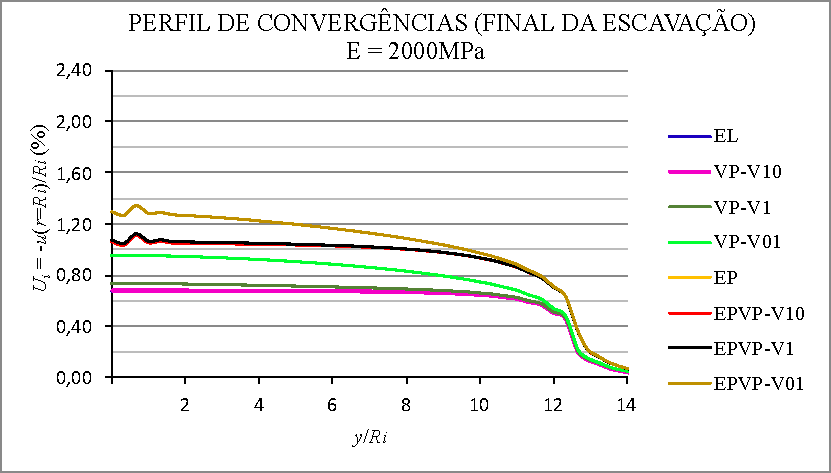
\includegraphics[scale = 1.0]{0719-PIEPI-E2000-FINALESCAVACAO.pdf}
	\end{center}
	\caption{\label{PIEPI-E2000-FINALESCAVACAO}Perfis de convergências no final da escavação para os diversos comportamentos implementados, considerando os parâmetros físicos do maciço de acordo com \citeonline{Piepi1995} com $E=2000$MPa}
\end{figure}

\begin{figure}[H]
	\begin{center}
		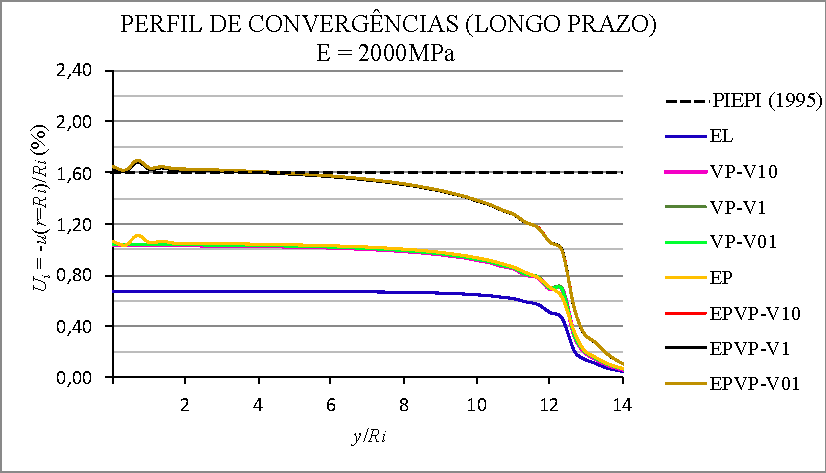
\includegraphics[scale = 1.0]{0720-PIEPI-E2000-LONGOPRAZO.pdf}
	\end{center}
	\caption{\label{PIEPI-E2000-LONGOPRAZO}Perfil de convergências no longo prazo para os diversos comportamentos implementados, considerando os parâmetros físicos do maciço de acordo com \citeonline{Piepi1995} com $E=2000$MPa}
\end{figure}

Os mesmos resultados foram obtidos utilizando o modelo 3D. A \autoref{PIEPI-E1500-CAMPO_DESLOCAMENTO} mostra o campo de deslocamentos no longo prazo para o caso (EPVP) com velocidade de escavação $V_p=0,1$m/dia e $E=1500$MPa.

\begin{figure}[H]
	\begin{center}
		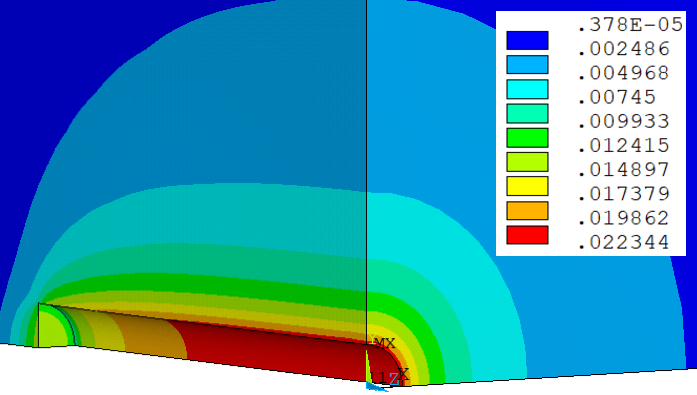
\includegraphics[scale = 1.0]{0721-PIEPI-E1500-CAMPO_DESLOCAMENTO.pdf
		}
	\end{center}
	\caption{\label{PIEPI-E1500-CAMPO_DESLOCAMENTO}Campo de deslocamentos no longo prazo para o caso elastoplástico-viscoplástico com $E=1500$MPa e $V_p=0,1$m/dia}
\end{figure}

A \autoref{PIEPI-E1500-CAMPO_DEFORMACOES} mostra o campo de deformações plásticas e viscosas equivalentes para o mesmo caso.

\begin{figure}[H]
	\begin{center}
		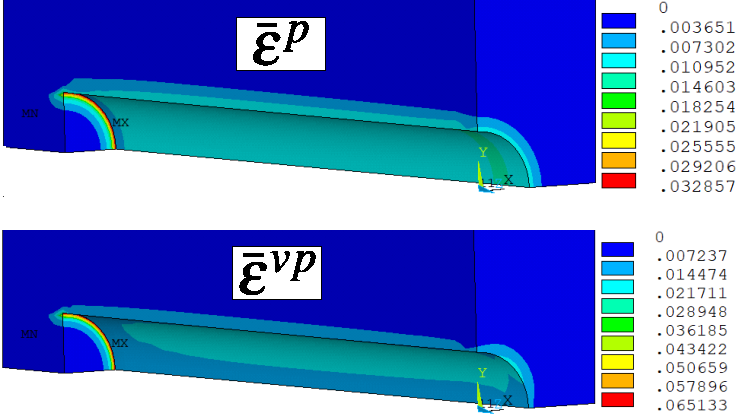
\includegraphics[scale = 1.0]{0722-PIEPI-E1500-CAMPO_DEFORMACOES.pdf
		}
	\end{center}
	\caption{\label{PIEPI-E1500-CAMPO_DEFORMACOES}Campo de deformações plásticas e viscosas no longo prazo para o caso elastoplástico-viscoplástico com $E=1500$MPa e $V_p=0,1$m/dia}
\end{figure}

\section{Verificação do modelo elastoplástico-viscoplástico com uma solução numérica}

\citeonline{Piepi1995} também desenvolveu sua solução numérica em axissimetria para verificar seus resultados analíticos e fazer estudos considerando a colocação do revestimento. Portanto, nesse aspecto, é possível também verificar o modelo desenvolvido com um de seus cálculos numéricos. Dessa forma tendo as propriedades $E=1500$MPa, $\nu=0,498$, $c^i=c^p=c^r =4\sqrt{3}/2$MPa, $c^{vp}=2\sqrt{3}/2$MPa, $\eta = 4 \cdot 10^4$dia, $n=1$, $f_0=1$MPa e $p_v=p_h=9$MPa, considerando um $E_{rev} = 2968,1$MPa, $d_0 = 2L_p$ e $V_p=12,5$m/dia \cite[p. 128, 132]{Piepi1995}, tem-se na \autoref{VP_COMPARAÇÃO_SOLUÇÃO_NUMÉRICA_CONVERGENCIA} e \autoref{EPVP_COMPARAÇÃO_SOLUÇÃO_NUMÉRICA_CONVERGENCIA} a comparação para o modelo viscoplástico (VP) e elastoplástico-viscoplástico (EPVP).

\begin{figure}[H]
	\begin{center}
		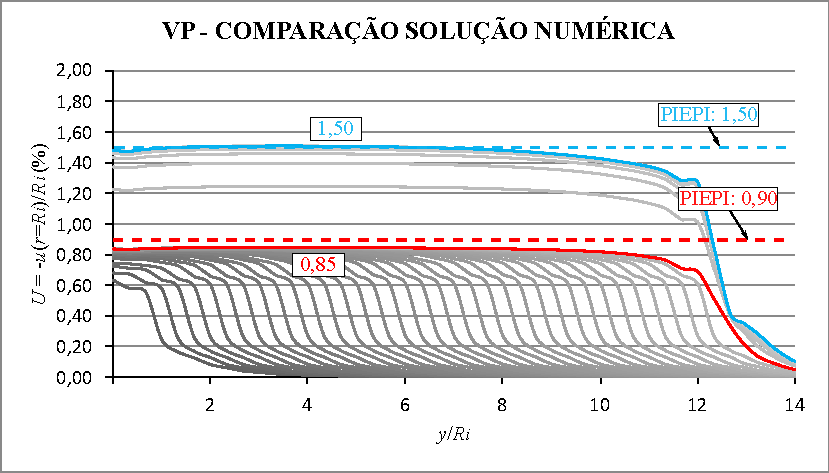
\includegraphics[scale = 1]{0723-VP_COMPARAÇÃO_SOLUÇÃO_NUMÉRICA_CONVERGENCIA.pdf}
	\end{center}
	\caption{\label{VP_COMPARAÇÃO_SOLUÇÃO_NUMÉRICA_CONVERGENCIA}Verificação com a solução de \citeonline{Piepi1995} do modelo viscoplástico com revestimento}
\end{figure}

\begin{figure}[H]
	\begin{center}
		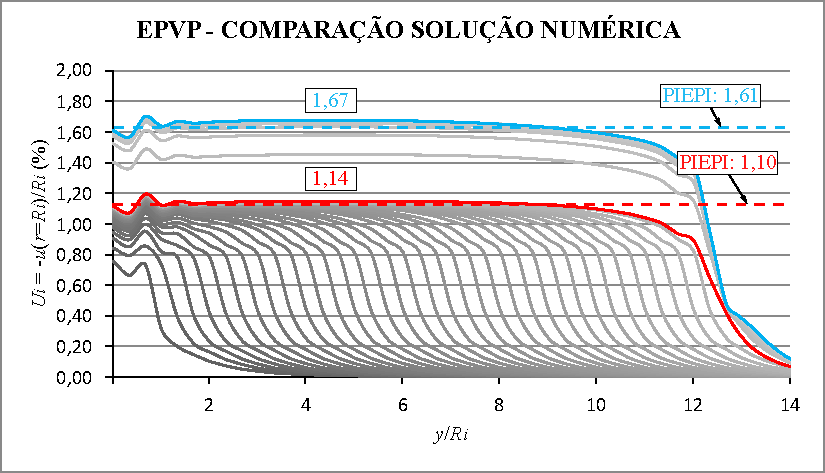
\includegraphics[scale = 1]{0724-EPVP_COMPARAÇÃO_SOLUÇÃO_NUMÉRICA_CONVERGENCIA.pdf}
	\end{center}
	\caption{\label{EPVP_COMPARAÇÃO_SOLUÇÃO_NUMÉRICA_CONVERGENCIA}Verificação com a solução de \citeonline{Piepi1995} do modelo elastoplástico-viscoplástico com revestimento}
\end{figure}

Pode-se notar que, para essas propriedades, o modelo elastoplástico-viscoplástico possuí uma convergência 34\% maior, no final da construção do túnel, e 11\% maior no longo prazo) em comparação com o modelo viscoplástico.

\section{Análise considerando amolecimento}

Como o modelo constitutivo elastoplástico-viscoplástico comporta a característica de endurecimento/amolecimento, nessa seção é apresentada uma pequena análise da influência que se pode ter em considerar esse fenômeno. Para tanto, é utilizado o exemplo anterior em axissimetria com as seguintes propriedades para o maciço: $E=1500$MPa, $\nu=0.498$, $c^{vp}=3\sqrt{3}/2$MPa, $\eta = 4 \cdot 10^4$dia, $n=1$, $f_0=1$MPa e $p_v=p_h=9$MPa. Vendo o campo de deformações plásticas equivalentes da \autoref{PIEPI-E1500-CAMPO_DEFORMACOES}, vamos adotar uma coesão inicial $c_i=4\sqrt{3}/2$MPa, contudo, um amolecimento linear até $\bar \varepsilon^p_{I} = 0,02$, para metade da coesão $c_p=2\sqrt{3}/2$MPa (\autoref{AMOLECIMENTO}).

Piepi também desenvolveu o seu modelo numérico em axissimetria. Nesse

\begin{figure}[H]
	\begin{center}
		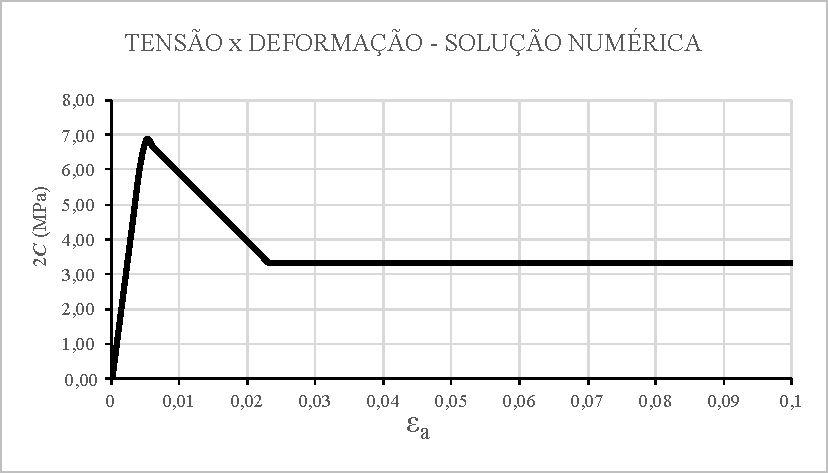
\includegraphics[scale = 0.8]{0725-AMOLECIMENTO.pdf
		}
	\end{center}
	\caption{\label{AMOLECIMENTO}Curva tensão \textit{versus} deformação obtido pelo modelo com amolecimento}
\end{figure}

A \autoref{EP-EFEITO-AMOLECIMENTO} mostra a diferença entre os perfis de convergências com amolecimento (C/AMOL) e sem (S/AMOL) para o modelo elastoplástico.

\begin{figure}[H]
	\begin{center}
		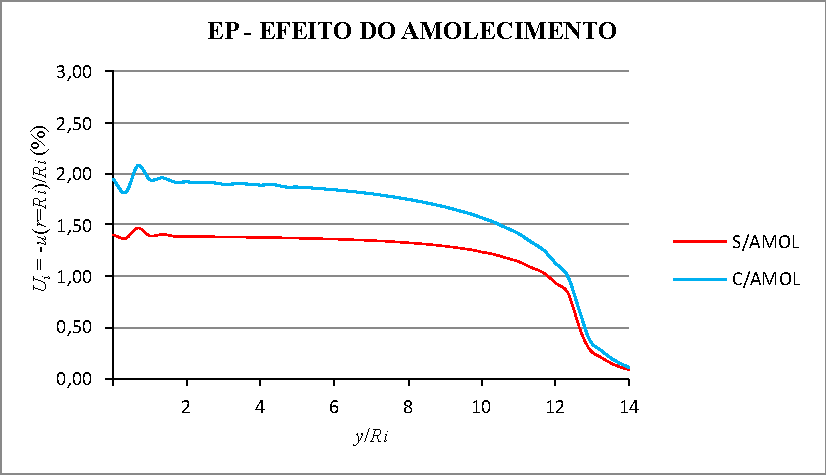
\includegraphics[scale = 1.0]{0726-EP-EFEITO-AMOLECIMENTO.pdf
		}
	\end{center}
	\caption{\label{EP-EFEITO-AMOLECIMENTO}Efeito do amolecimento no perfil de convergências para o caso elastoplástico}
\end{figure}

A \autoref{EPVP-EFEITO-AMOLECIMENTO} mostra a diferença entre os perfis de convergências com e sem amolecimento para o modelo elastoplástico-viscoplástico no final da construção do túnel, ou seja, no curto prazo (CP) e no longo prazo (LP). É adotado uma velocidade $V_p=0,1$m/dia.

\begin{figure}[H]
	\begin{center}
		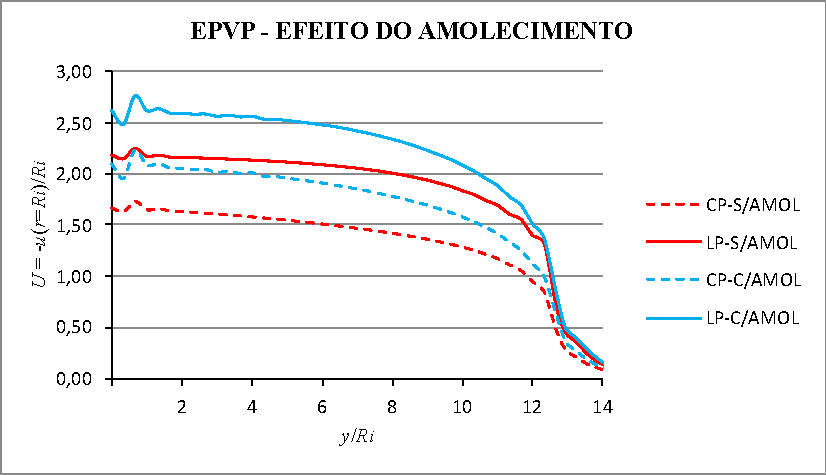
\includegraphics[scale = 1.0]{0725-EPVP-EFEITO-AMOLECIMENTO.pdf}
	\end{center}
	\caption{\label{EPVP-EFEITO-AMOLECIMENTO}Efeito do amolecimento no perfil de convergências para o caso elastoplástico-viscoplástico}
\end{figure}

Para o modelo elastoplástico, a redução na coesão pela metade devido ao amolecimento se traduziu em uma convergência 37\% maior. Já para o modelo elastoplástico-viscoplástico, no final da construção do túnel (curto prazo) o amolecimento representou um aumento de 28\% e no longo prazo de 24\%.


\section{Análise paramétrica da influência do revestimento}

Nessa seção é apresentada uma análise paramétrica para averiguar a influência do revestimento sobre o perfil de convergência do modelo elastoplástico-viscoplástico. As propriedades do maciço são as mesmas da análise anterior com $E=1500$MPa. É utilizado o modelo em axissimetria, primeiramente sem revestimento e então com revestimento variando o seu módulo de elasticidade de $E_{rev} = 3000$MPa para $E_{rev} = 30000$MPa e a distância não suportada de $d0 = 0$ e de $d0 = 4L_p$. A \autoref{PARAMETRICO-D0-FINALCONSTRUÇÃO} e \autoref{PARAMETRICO-D0-LONGOPRAZO} mostram os resultados considerando $d_0 = 0$ e a \autoref{PARAMETRICO-D4-FINALCONSTRUÇÃO} e \autoref{PARAMETRICO-D4-LONGOPRAZO} considerando $d_0=4L_p$. A convergência ao equilíbrio é medida em $y/R_i = 6$. 

Quando a rigidez do revestimento é alta o modelo (VP) se aproxima do (EL). Isso ocorre, pois as deformações viscosas do modelo viscoplástico são resistidas pelo revestimento e impedidas de ocorrer. Já o modelo (EPVP) se aproxima do (EP). Isso, pois durante a escavação e colocação do revestimento, alguma plastificação ocorre, mas as deformações viscosas do modelo (EPVP) são resistidas pelo revestimento.

Comparando o modelo elastoplástico-viscoplástico com o modelo viscoplástico, no final da construção, sem revestimento, o primeiro teve uma convergência 33\%. Com revestimento aplicado a $d0=0$ uma convergência entre 17\% e 20\% e para $d0=4L_p$ entre 25\% a 28\% maior. No longo prazo, sem revestimento, o primeiro teve, uma convergência 54\% maior. Com revestimento aplicado a $d0=0$ uma convergência entre 17\% e 23\% e para $d0=4L_p$ entre 26\% a 30\% maior. Isso é uma grande diferença com relação a modelos que procuram estimar a convergência no longo prazo, mas não consideram a plastificação do maciço no comportamento instantâneo.

\begin{figure}[H]
	\begin{center}
		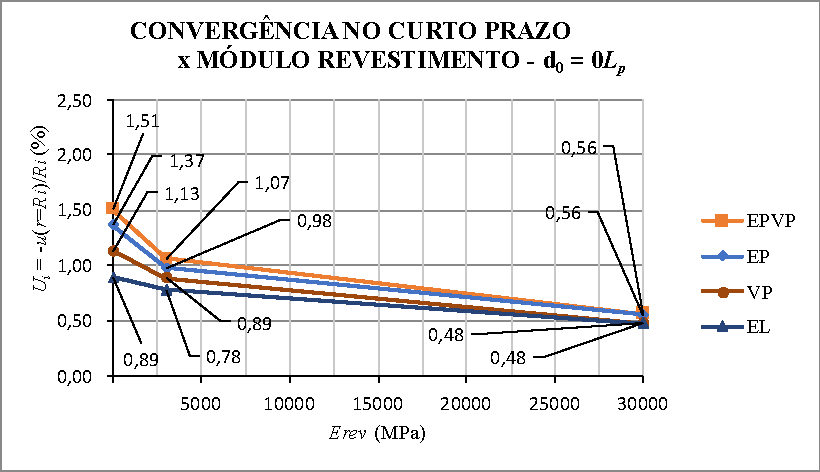
\includegraphics[scale = 1.0]{0728-PARAMETRICO-D0-FINALCONSTRUÇÃO.pdf
		}
	\end{center}
	\caption{\label{PARAMETRICO-D0-FINALCONSTRUÇÃO}Convergência no final da construção \textit{versus} módulo de elasticidade do revestimento para uma distância não revestida $d0=0$}
\end{figure}

\begin{figure}[H]
	\begin{center}
		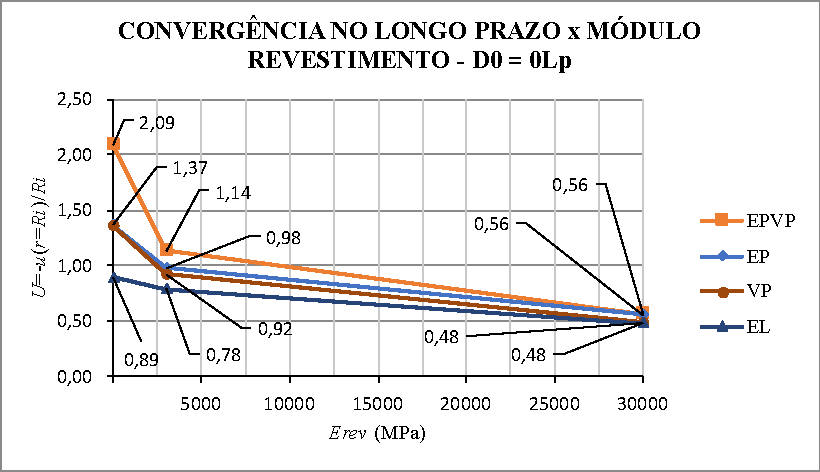
\includegraphics[scale = 1.0]{0729-PARAMETRICO-D0-LONGOPRAZO.pdf
		}
	\end{center}
	\caption{\label{PARAMETRICO-D0-LONGOPRAZO}Convergência no longo prazo \textit{versus} módulo de elasticidade do revestimento para uma distância não revestida $d0=0$}
\end{figure}

\begin{figure}[H]
	\begin{center}
		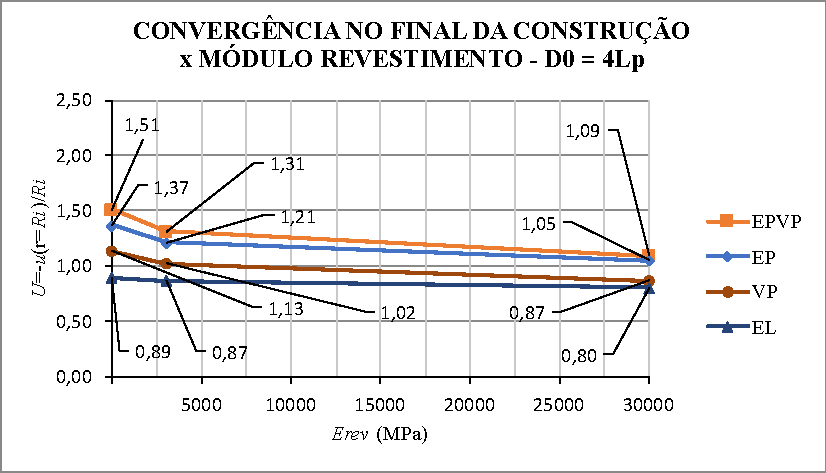
\includegraphics[scale = 1.0]{0730-PARAMETRICO-D4-FINALCONSTRUÇÃO.pdf
		}
	\end{center}
	\caption{\label{PARAMETRICO-D4-FINALCONSTRUÇÃO}Convergência no final da construção \textit{versus} módulo de elasticidade do revestimento para uma distância não revestida $d0=4L_p$}
\end{figure}

\begin{figure}[H]
	\begin{center}
		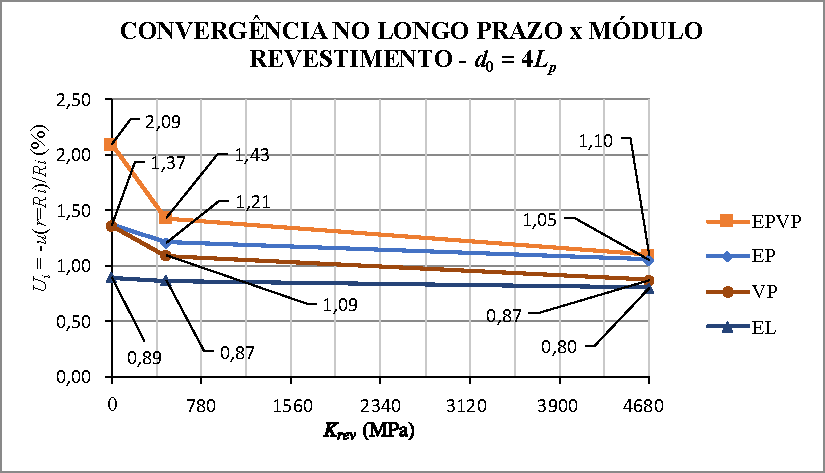
\includegraphics[scale = 1.0]{0731-PARAMETRICO-D4-LONGOPRAZO.pdf
		}
	\end{center}
	\caption{\label{PARAMETRICO-D4-LONGOPRAZO}Convergência no longo prazo \textit{versus} módulo de elasticidade do revestimento para uma distância não revestida $d0=4L_p$}
\end{figure}

\section{Análise paramétrica considerando uma seção elíptica}

Uma vez que o modelo constitutivo acoplado (EPVP) está generalizado para o caso tridimensional é interessante fazer uma análise paramétrica considerando algum aspecto que não pode ser analisado com o modelo axissimétrico. O aspecto escolhido nessa análise foi a razão entre o raio horizontal e vertical. Dessa forma, foram consideradas duas razões de aspecto $R_{h_i}/R_{vi}$: 1, ou seja, circular e 2. Além disso, os cálculos foram executados sem revestimento (S/REV) e com revestimento (C/REV) afastado de $d0=2L_p$ da face de escavação. As propriedades do maciço são: $E=1500$MPa, $\nu=0,498$, $c^i=c^p=c^r =4\sqrt{3}/2$MPa, $c^{vp}=2\sqrt{3}/2$MPa, $\eta = 4 \cdot 10^4$dia, $n=1$, $f_0=1$MPa e $p_v=p_h=9$MPa. E do revestimento: $E_{rev}=2968.1$MPa, $\nu_{rev}$=0,3 com uma velocidade de escavação e colocação de $V_p=1$m/dia. Para evidenciar a diferença que o modelo acoplado pode representar os resultados foram comparados com modelo viscoplástico (VP) com uma coesão de $2\sqrt{3}/2$MPa.

Como a seção transversal é eliptica as convergências são medidas ao longo do maior e menor eixo da seção, portanto,  tem-se $U_{yi} = -u_y(r=R_{vi})/R_{vi}$ e $U_{xi} = -u_x(r=R_{hi})/R_{hi}$.  A \autoref{ELIPTICO-CONVERGENCIAS-UX-SREV} e \autoref{ELIPTICO-CONVERGENCIAS-UX-CREV} mostram as convergências no equilíbrio na direção $x$ para ambos os modelos (VP) e (EPVP), no curto prazo (CP), ou seja, no final da construção do túnel e no longo prazo (LP) sem revestimento e com revestimento, respectivamente.


\begin{figure}[H]
	\begin{center}
		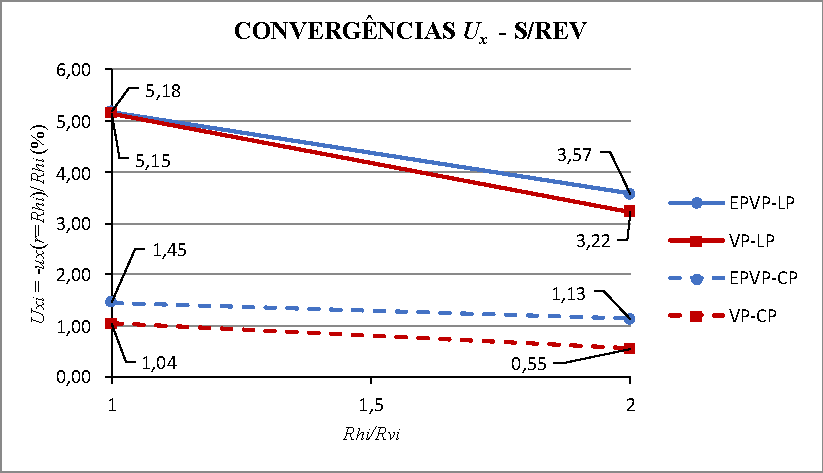
\includegraphics[scale = 1.0]{0732-ELIPTICO-CONVERGENCIAS-UX-SREV.pdf
		}
	\end{center}
	\caption{\label{ELIPTICO-CONVERGENCIAS-UX-SREV}Convergências na direção $x$ \textit{versus} razão de aspecto da seção sem revestimento}
\end{figure}

\begin{figure}[H]
	\begin{center}
		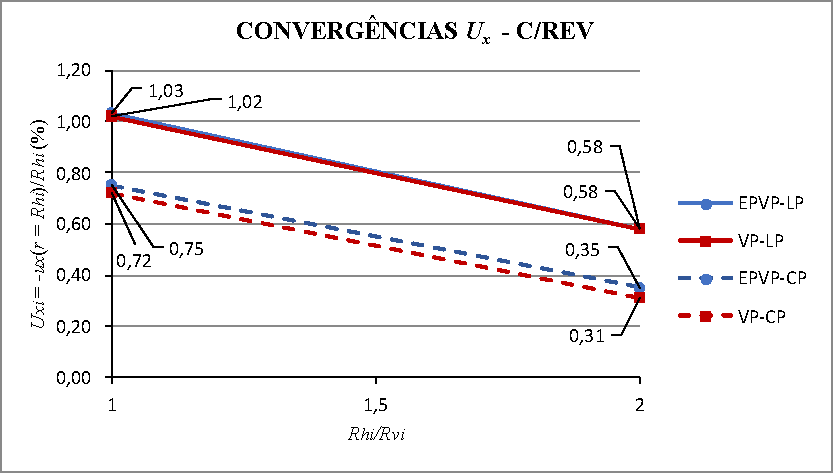
\includegraphics[scale = 1.0]{0733-ELIPTICO-CONVERGENCIAS-UX-CREV.pdf
		}
	\end{center}
	\caption{\label{ELIPTICO-CONVERGENCIAS-UX-CREV}Convergências na direção $x$ \textit{versus} razão de aspecto da seção com revestimento}
\end{figure}

De uma forma geral, quando se aumenta a razão de aspecto os deslocamentos $u_x$ aumentam. Contudo, a convergência diminui, pois, está sendo dividida pelo raio horizontal do túnel. De qualquer forma, pode-se ver, ao comparar, a \autoref{ELIPTICO-CONVERGENCIAS-UX-SREV} com a \autoref{ELIPTICO-CONVERGENCIAS-UX-CREV} a influência significativa do revestimento nas convergências. Sem revestimento uma maior razão de aspecto leva a maiores convergências do modelo (EPVP) e isso é esperado uma vez que nessa borda, contígua ao eixo $x$, tem-se as maiores plastificações. O revestimento, contudo, bloqueia a maior parte dessas deformações plásticas, fazendo com que tenha apenas as deformações viscosas e dessa forma, ambas as curvas (VP) e (EPVP) se aproximam no longo prazo. 

A \autoref{ELIPTICO-CONVERGENCIAS-UX-SREV} e \autoref{ELIPTICO-CONVERGENCIAS-UX-SREV} mostra as convergências ao equilíbrio para a direção $y$. Nesse caso, no longo prazo, não há diferença entre os modelos. Isso ocorre, pois, nessa direção, apesar de se ter as maiores convergências, não há plastificações tão significativas conforme a razão de aspecto aumenta. Isso faz com que ambas as curvas deem o mesmo resultado no longo prazo, tanto sem quanto com revestimento. Isso pode ser verificado pelo nível de plastificação que ocorre na seção. A Figura XX mostra o campo de deformações inelásticas equivalentes comparando o modelo (VP) e (EPVP), sem revestimento, com razão de aspecto 2 e no longo prazo.

\begin{figure}[H]
	\begin{center}
		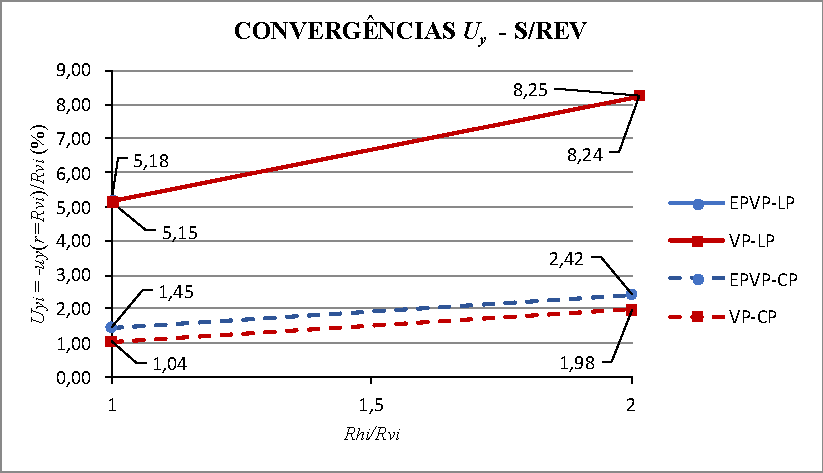
\includegraphics[scale = 1.0]{0734-ELIPTICO-CONVERGENCIAS-UY-SREV.pdf
		}
	\end{center}
	\caption{\label{ELIPTICO-CONVERGENCIAS-UY-SREV}Convergências na direção $y$ \textit{versus} razão de aspecto da seção sem revestimento}
\end{figure}

\begin{figure}[H]
	\begin{center}
		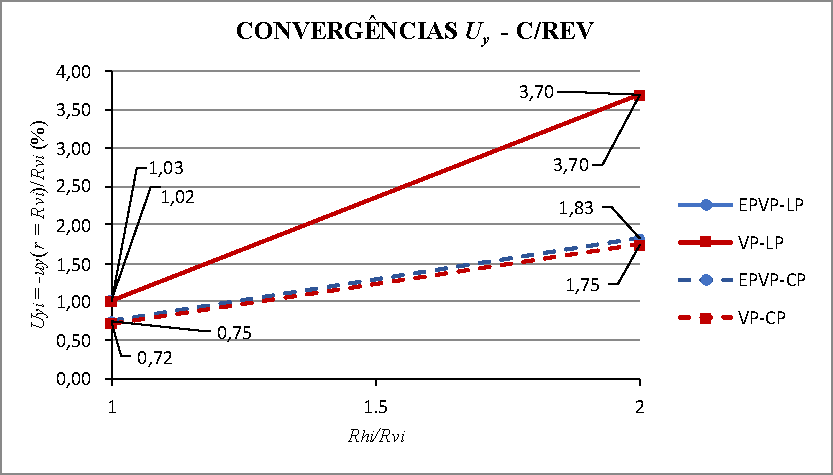
\includegraphics[scale = 1.0]{0735-ELIPTICO-CONVERGENCIAS-UY-CREV.pdf
		}
	\end{center}
	\caption{\label{ELIPTICO-CONVERGENCIAS-UY-CREV}Convergências na direção $y$ \textit{versus} razão de aspecto da seção com revestimento}
\end{figure}

\begin{figure}[H]
	\begin{center}
		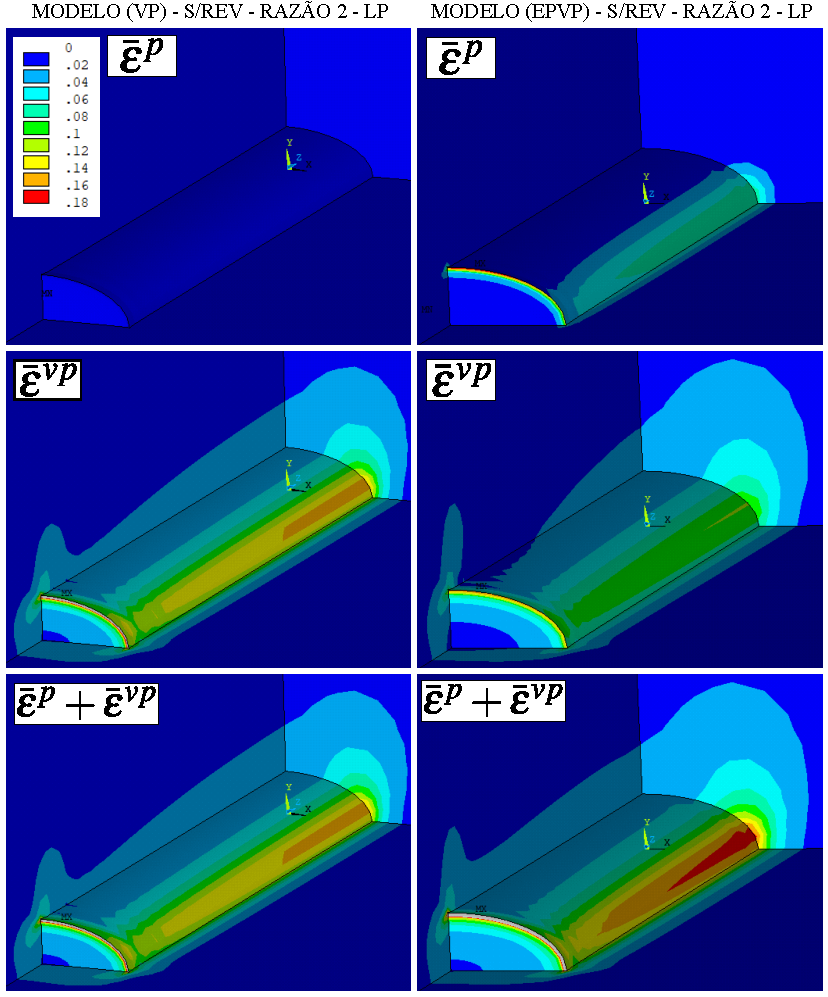
\includegraphics[scale = 1.0]{0736-campo_deformacoes_eliptico.pdf
		}
	\end{center}
	\caption{\label{ELIPTICO-CONVERGENCIAS-UY-SREV}Campo de deformações equivalentes para o modelo (VP) e (EPVP), sem revestimento, com razão de aspecto 2 e no longo prazo}
\end{figure}

A \autoref{convergencias_analise_secao_eliptica} resume a razão entre as convergências elastoplásticas-viscplástica e viscoplástica.

\begin{table}[H]
	\caption{Razão entre as convergências ao equilíbrio do modelo (EPVP) com (VP)}
	\label{convergencias_analise_secao_eliptica}
	\centering
	\small
	\renewcommand{\arraystretch}{1.25}
	\begin{tabular}{c c c c c}
		\hline
		\multicolumn{5}{c}{\textbf{EPVP / VP}}\\	
		\hline
		\multicolumn{1}{c}{} &
		\multicolumn{2}{c}{\textbf{CURTO PRAZO}} &
		\multicolumn{2}{c}{\textbf{LONGO PRAZO}}	\\
		\multicolumn{1}{c}{} &
		\multicolumn{1}{c}{\textbf{Ux}} &
		\multicolumn{1}{c}{\textbf{Uy}} &
		\multicolumn{1}{c}{\textbf{Ux}} &
		\multicolumn{1}{c}{\textbf{Uy}} \\
		\hline
		S/REV-R1	 &	1,39 &	1,39 &	1,01 &	1,01 \\
		S/REV-R2	 &	2,05 &	1,22 &	1,11 &	1,00 \\
		C/REV-R1	 &	1,04 &	1,04 &	1,01 &	1,01 \\
		C/REV-R2	 &	1,13 &	1,05 &	1,00 &	1,00 \\
		\hline
	\end{tabular}
	\normalsize
\end{table}

Como pode-se ver as maiores diferenças ocorrem sem a presença do revestimento. Mas isso porque houve uma contenção das deformações plásticas. Sem revestimento, para razão de aspecto 1, o modelo (EPVP) causa um aumento de 39\% na convergência. Sem revestimento, para a razão de aspecto 2, na direção $x$, tem-se um aumento de 105\% (curto prazo) e 11\% (no longo prazo). E na direção $y$ um aumento no curto prazo de 22\%.

A \autoref{convergencias_analise_secao_eliptica_2} mostra a razão entre as convergências no equilíbrio de longo prazo e curto prazo para ambos os modelos em ambas direções.

\begin{table}[H]
	\caption{Razão entre as convergências no equilíbrio de longo prazo pelo curto prazo do modelo (VP) e (EPVP)}
	\label{convergencias_analise_secao_eliptica_2}
	\centering
	\small
	\renewcommand{\arraystretch}{1.25}
	\begin{tabular}{c c c c c}
		\hline
		\multicolumn{5}{c}{\textbf{LONGO PRAZO / CURTO PRAZO}}\\	
		\hline
		\multicolumn{1}{c}{} &
		\multicolumn{2}{c}{\textbf{VP}} &
		\multicolumn{2}{c}{\textbf{EPVP}}	\\
		\multicolumn{1}{c}{} &
		\multicolumn{1}{c}{\textbf{Ux}} &
		\multicolumn{1}{c}{\textbf{Uy}} &
		\multicolumn{1}{c}{\textbf{Ux}} &
		\multicolumn{1}{c}{\textbf{Uy}} \\
		\hline
		S/R-R1	 &	4,95 &	4,95 &	3,57 &	1,00 \\
		S/R-R2	 &	5,85 &	4,17 &	3,16 &	2,31 \\
		C/R-R1	 &	1,42 &	1,42 &	1,37 &	1,37 \\
		C/R-R2	 &	1,87 &	2,11 &	1,66 &	2,02 \\
		\hline
	\end{tabular}
	\normalsize
\end{table}

Pode-se ver que nesse caso, o modelo (EPVP) apresentou menores relações. Isso é esperado, uma vez que, algum nível de plastificação ocorre no curto prazo.




